\documentclass[../../main.tex]{subfiles}
    
    \lstset{basicstyle=\small,
      showstringspaces=false,
      commentstyle=\color{black},
      keywordstyle=\color{blue}
    }
    
    \graphicspath{{images/Antrieb/}{../../images/Antrieb/}}

    \begin{document}
    \subsection{Antrieb}
    In der Anforderungsliste sind diverse Anforderungen an den Antrieb des Zuges gefordert.
    Der Zug soll einerseits möglichst Schnell fahren können, muss aber auch präzise angesteuert werden können um die Geschwindigkeit je nach Situation anpassen zu können und präzise anzuhalten.
    Die Möglichkeiten sind dabei durch die Anforderungen etwas eingeschränkt wie z.B. mit der Strombegrenzug von 3A.
    In diesem Kaptitel werden verschiedene Konzepte beschrieben und analysiert.

    \textbf{Übersicht Konzepte}\\
    Es werden der verschiedene Elektromotoren betrachtet. Zu jeder Möglichkeit werden Vor- und Nachteile aufgelistet und Risiken analysiert.

    \begin{itemize}
        \item DC-Motor Bürstenlos
        \item DC-Motor Bürstenbehaftet
        \item Schrittmotor
    \end{itemize}

    \subsubsection{DC-Motor Bürstenlos}
    %Quelle: https://de.nanotec.com/support/knowledge-base-pages/animation-buerstenlose-dc-motoren/?tx_nanotec_animation%5Binitial%5D=motor_bldc_block_delta&cHash=16dd715993449effcf3951fe40aaa206

    Bürstenlose DC-Motoren (auch als EC-Motor bezeichnet) werden normalerweise mit 3 Phasen angesteuert. Dadurch ist kein Kommutator mit Schleifkontakten notwendig. Dies macht den Motor zuverlässiger, da kein Verschleiss durch die Schleifkontakte entsteht.
    Die Konsequenz dieser Ansteuerung ist jedoch, dass diese Motoren nicht direkt von einem Mikrocontroller angesteuert werden können. Es ist eine Steuerung als Treiber nötig. Diese ist oftmals durch den Hersteller vorgegeben oder Empfolen.

    \begin{flushleft}
        \begin{table}[H]
        \begin{tabular}{ | l | p{11cm} |}
        \hline
        \textbf{Problemstellung} & Antrieb \\ \hline
        \textbf{Disziplin} & Elektrotechnik \\ \hline
        \textbf{Lösungskonzept} & DC-Motor Bürstenlos\\ \hline
        \textbf{Komponente} & \begin{itemize}
            \item DC-Motor Maxon EC 45 flat
            \item Steuerung - DEC Module
            \end{itemize}\\ \hline
        \textbf{Bewertung} &  \begin{itemize}
                                \item[+] kleiner Platzbedarf mit Flachmotor
                                \item[+] Qualitativ guter Motor
                                \item[+] hohe Umdrehungszahl möglich 
                                \item[-] hohe Kosten 
                                \item[-] keine exakte Positionnierung mit günstigerer Steuerung
                              \end{itemize} \\ \hline
        \end{tabular}
        \caption{Konzeptbeurteilung: DC-Motor Bürstenlos}
        \label{tab:antr_konzept_dcMotor_buerstenlos}
    \end{table}
    \end{flushleft}

    \textbf{Risiken}\\
    Zu diesem Lösungskonzept werden folgende Risiken betrachtet und eingeschätzt.
    \begin{enumerate}[I]
        \item zu Tief begrenzte umdrehungszahl
        \item zu wenig Drehmoment
        \item zu Teuer
        \item zu wenig Präzise steuerung
        \item zu schwierige Umsetzung (unter Berücksichtigung einer späteren Änderung zu einer Alternativlösung)        
    \end{enumerate}

    In Abbildung \ref{fig:antr_risikomatrix_buerstenlos} werden die Risiken nach möglicher Schadenshöhe und Eintrittswahrscheinlichkeit eingeschätzt.

    \begin{figure}[H]
        \centering
        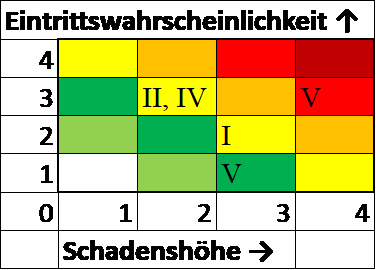
\includegraphics[width=0.4\textwidth]{Antr_Risiko_DCMotor_Buerstenlos.png}
        \caption {Risikomatrix DC-Motor Bürstenlos}
        \label{fig:antr_risikomatrix_buerstenlos}
    \end{figure}

    Hier ist besonders das Risiko der Umsetzung besonders gross. Dieses lässt sich durch den Einsatz einer guten Steuerung minimieren, diese sind jedoch sehr kostspielig.

    \subsubsection{DC-Motor Bürstenbehaftet}
    %Quelle: https://de.wikipedia.org/wiki/Gleichstrommaschine
    
    Bürstenbehaftete DC-Motoren sind das was traditionnell als 'Gelichstrommaschiene' bezeichnet wird. Mit Schleifkontakten wird die Rotorenwicklung beim Drehen umgepolt.
    Bei Bürstenbehafteten DC-Motoren ist es möglich die Geschwindigkeit durch verändern der Spannung oder durch ansteuerung mit einem PWM einzustellen. Die Drehrichtung wird durch die Polarität festgelegt.

    \begin{flushleft}
        \begin{table}[H]
        \begin{tabular}{ | l | p{11cm} |}
        \hline
        \textbf{Problemstellung} & Antrieb \\ \hline
        \textbf{Disziplin} & Elektrotechnik \\ \hline
        \textbf{Lösungskonzept} & DC-Motor Bürstenbehaftet\\ \hline
        \textbf{Komponente} & \begin{itemize}
            \item DC-Motor ... TODO
            \item Steuerung / Treiber (H-Brücke)
            \end{itemize}\\ \hline
        \textbf{Bewertung} &  \begin{itemize}
                                \item[+] hohe Umdrehungszahl möglich 
                                \item[+] Kostengünstig 
                                \item[+] Einfache ansteuerung vom Mikrocontroller via PWM 
                                \item[-] keine exakte Positionnierung
                                \item[-] grosser Platzbedarf
                              \end{itemize} \\ \hline
        \end{tabular}
        \caption{Konzeptbeurteilung: DC-Motor Bürstenbehaftet}
        \label{tab:antr_konzept_dcMotor_buerstenbehaftet}
    \end{table}
    \end{flushleft}

    \textbf{Risiken}\\
    Zu diesem Lösungskonzept werden folgende Risiken betrachtet und eingeschätzt.
    \begin{enumerate}[I]
        \item zu Tief begrenzte umdrehungszahl
        \item zu wenig Drehmoment
        \item zu Teuer
        \item zu wenig Präzise steuerung
        \item zu schwierige Umsetzung (unter Berücksichtigung einer späteren Änderung zu einer Alternativlösung)  
    \end{enumerate}

    In Abbildung \ref{fig:antr_risikomatrix_buerstenbehaftet} werden die Risiken nach möglicher Schadenshöhe und Eintrittswahrscheinlichkeit eingeschätzt.

    \begin{figure}[H]
        \centering
        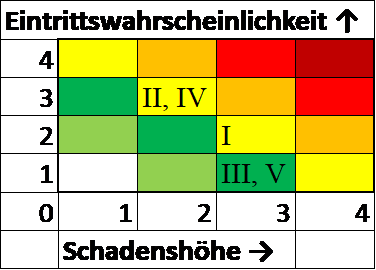
\includegraphics[width=0.4\textwidth]{Antr_Risiko_DCMotor_Buerstenbehaftet.png}
        \caption {Risikomatrix DC-Motor Bürstenbehaftet}
        \label{fig:antr_risikomatrix_buerstenbehaftet}
    \end{figure}

    Die Risiken im gelben bereich lassen sich mit einer sorgfältigen Auslegung und richtiger Ansteuerung des Motors minimieren. Bei diesem Konzept müssen diese Punkte also speziell in der Planung und auswahl beachtet werden. 

    \subsubsection{Schrittmotor}
    %Quelle: https://de.wikipedia.org/wiki/Schrittmotor
    Bei Schrittmotoren wird das Magnetfeld im Stator schrittweise gedreht. Dadurch lässt sich die Position mit einem bestimten Winkel vorgeben.

    \begin{flushleft}
        \begin{table}[H]
        \begin{tabular}{ | l | p{11cm} |}
        \hline
        \textbf{Problemstellung} & Antrieb \\ \hline
        \textbf{Disziplin} & Elektrotechnik \\ \hline
        \textbf{Lösungskonzept} & Schrittmotor\\ \hline
        \textbf{Komponente} & \begin{itemize}
            \item Motor ... TODO
            \item Steuerung ... TODO
            \end{itemize}\\ \hline
        \textbf{Bewertung} &  \begin{itemize} 
                                \item[+] exakte Positionnierung möglich
                                \item[-] keine grosse Drehzahl möglich
                                \item[-] grosser Platzbedarf
                              \end{itemize} \\ \hline
        \end{tabular}
        \caption{Konzeptbeurteilung: Schrittmotor}
        \label{tab:antr_konzept_schrittmotor}
    \end{table}
    \end{flushleft}
    

    \textbf{Risiken}\\
    Zu diesem Lösungskonzept werden folgende Risiken betrachtet und eingeschätzt.
    \begin{enumerate}[I]
        \item zu Tief begrenzte umdrehungszahl
        \item zu wenig Drehmoment
        \item zu Teuer
        \item zu wenig Präzise steuerung
        \item zu schwierige Umsetzung (unter Berücksichtigung einer späteren Änderung zu einer Alternativlösung)        
    \end{enumerate}

    In Abbildung \ref{fig:antr_risikomatrix_schrittmotor} werden die Risiken nach möglicher Schadenshöhe und Eintrittswahrscheinlichkeit eingeschätzt.

    \begin{figure}[H]
        \centering
        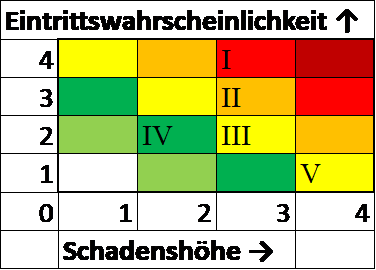
\includegraphics[width=0.4\textwidth]{Antr_Risiko_Schrittmotor.png}
        \caption {Risikomatrix Schrittmotor}
        \label{fig:antr_risikomatrix_schrittmotor}
    \end{figure}

    Hier ist besonders die Dimensionierung des Motors eine grosses Risiko. Das Risiko der zu geringen Drehzahl lässt sich mit einer Mechanischen Lösung  minimieren. Um das Risiko der zu geringen Drehzahl zu minimieren muss der Motor entsprechend stark dimensioniert werden. Dies erhöht jedoch auch wider die Kosten, den Platzbedarf und den Stromverbrauch.

    \subsubsection{Entscheid}
    Mithilfe der Nutzwertanalyse in Abbildung \ref{fig:antr_nutzwertanalyse} konnte ein Entscheid getroffen werden.\\
    Der Bürstenlo DC-Motor wurde mit dem grössten Nutzen bewertet. Vorallem die kleine Bauart und die Präzision ist ein grosses Argument für den Bürstenlosen DC-Motor.\\
    Der Bürstenbehaftet DC-Motor fällt vorallem durch die grössere Bauart und das grössere Gewicht ab. Jedoch ist er für die Umsetzung und auch vom Preis her viel attraktiver.\\
    Der Schrittmotor fiel ebenfalls bei der Grösse und beim Gewicht ab. Jedoch bietet der Schrittmotor keinen grossen Vorteil was die Einfachheit der Umsetzung angeht. Deshalb erreicht er die Schlechteste Bewertung in dieser Analyse.\\
        
    \begin{figure}[H]
        \centering
        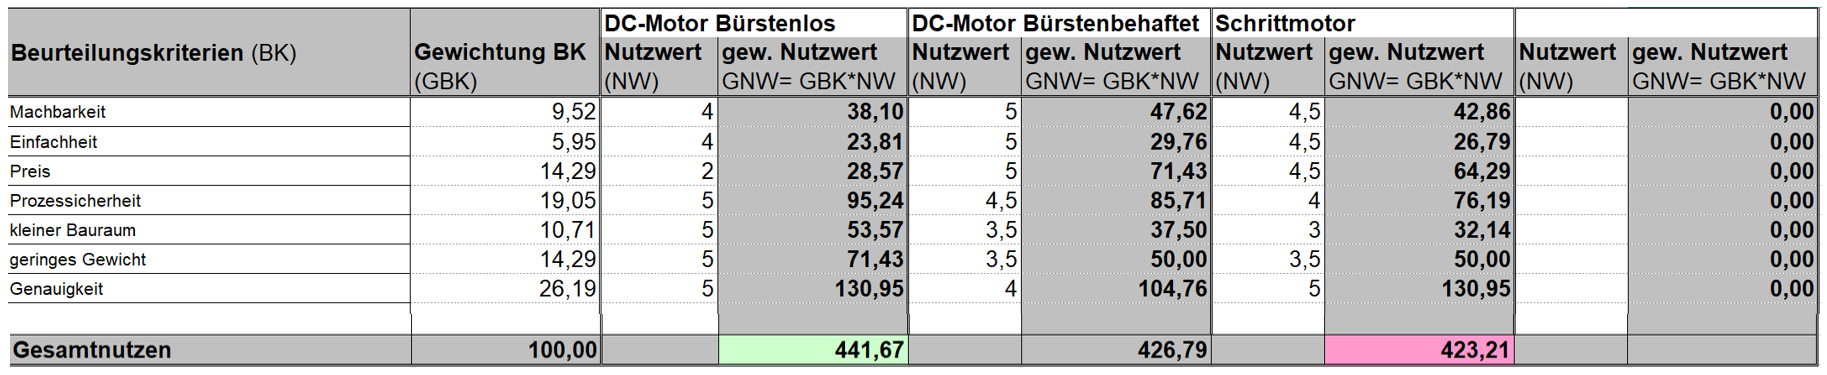
\includegraphics[width=1.0\textwidth]{Antr_Nutzwertanalyse.png}
        \caption {Nutzwertanalyse Antrieb}
        \label{fig:antr_nutzwertanalyse}
    \end{figure}

    Der Entscheid im Morphologischen Kasten fiel Schlussendlich auf den Bürstenbehafteten DC-Motor. Der Grund dass die Entscheidung entgegen der Nutzwertanalyse fiel ist, dass der grosse Preis zusammen mit der anspruchsvollen Umsetzung beim Bürstenlosen DC-Motor ein zu grosses Risiko ist. Das Risiko der Baugrösse und des Gewichtes des Bürstenbehafteten Motors kann durch eine grosszügige Auslegung der Mechanik minimiert werden.\\
    Der Bürstenlose DC-Motor wird als Alternativlösung im Plan B weiter verfolgt für den Fall dass die Anforderungen mit dem Bürstenbehafteten Motor nicht erfüllt werden können. Weitere Tests in der Entwicklung des Konzeptes werden dies zeigen.

    \end{document}